% =====================================================================
%  Capítulo 4 — Implementação
% =====================================================================
\chapter{Implementação}
\label{cap:implementacao}
\rubricaFuncionalidade

\section{Montagem}

O protótipo continua numa protoboard. O ESP32 DevKit V1 ocupa as linhas
A a I, na posição mais à esquerda, com o conector USB para fora e a
trilha azul (GND) para baixo. O DHT11 fica em J45 e o BH1750 em J55--59,
no lugar do antigo módulo fotorresistor. Todas as ligações usam fios
macho-macho. A Figura~\ref{fig:montagem} mostra o esquema, e a
Tabela~\ref{tab:ligacoes} lista cada fio como está na bancada
(\caminho{firmware/intrucoes_montagem.md}).

\begin{figure}[H]
\centering
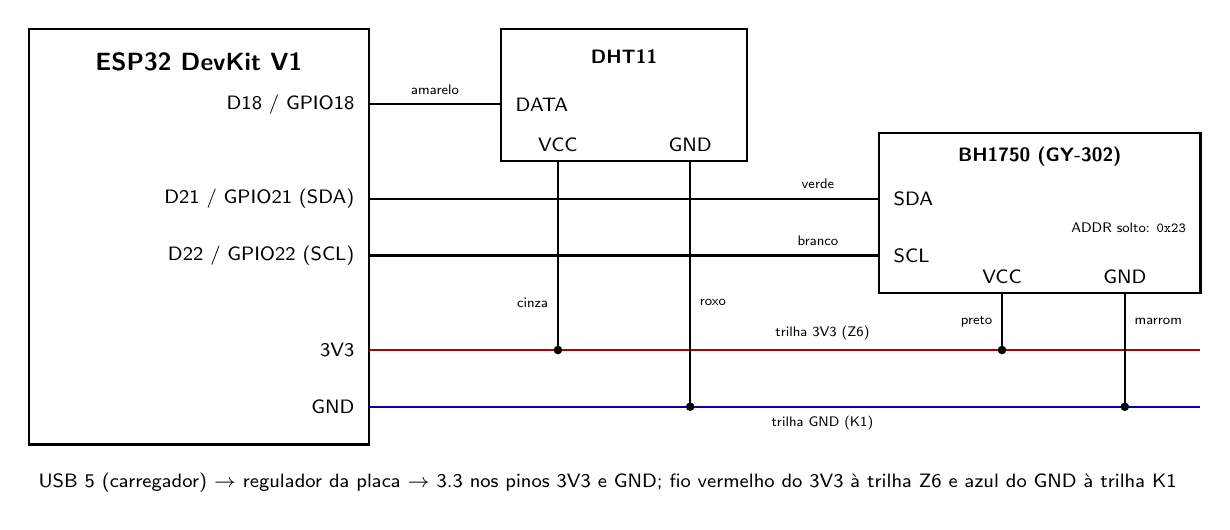
\begin{tikzpicture}[x=1.2cm, y=1.2cm, font=\sffamily\scriptsize,
  fio/.style={thick},
  cor/.style={font=\sffamily\tiny},
  no/.style={circle, fill, inner sep=1.1pt}]
  % ESP32: pinos na borda direita
  \draw[thick] (0,0) rectangle (3.6,4.4);
  \node[font=\sffamily\small\bfseries] at (1.8,4.05) {ESP32 DevKit V1};
  \node[anchor=east] at (3.55,3.6) {D18 / GPIO18};
  \node[anchor=east] at (3.55,2.6) {D21 / GPIO21 (SDA)};
  \node[anchor=east] at (3.55,2.0) {D22 / GPIO22 (SCL)};
  \node[anchor=east] at (3.55,1.0) {3V3};
  \node[anchor=east] at (3.55,0.4) {GND};
  % DHT11
  \draw[thick] (5.0,3.0) rectangle (7.6,4.4);
  \node[font=\sffamily\scriptsize\bfseries] at (6.3,4.1) {DHT11};
  \node[anchor=west] at (5.05,3.6) {DATA};
  \node[anchor=south] at (5.6,3.0) {VCC};
  \node[anchor=south] at (7.0,3.0) {GND};
  % BH1750
  \draw[thick] (9.0,1.6) rectangle (12.4,3.3);
  \node[font=\sffamily\scriptsize\bfseries] at (10.7,3.05) {BH1750 (GY-302)};
  \node[anchor=west] at (9.05,2.6) {SDA};
  \node[anchor=west] at (9.05,2.0) {SCL};
  \node[anchor=south] at (10.3,1.6) {VCC};
  \node[anchor=south] at (11.6,1.6) {GND};
  \node[anchor=east, cor] at (12.35,2.3) {ADDR solto: \texttt{0x23}};
  % Sinais
  \draw[fio] (3.6,3.6) -- node[cor, above]{amarelo} (5.0,3.6);
  \draw[fio] (3.6,2.6) -- (9.0,2.6) node[cor, above, pos=0.88]{verde};
  \draw[fio] (3.6,2.0) -- (9.0,2.0) node[cor, above, pos=0.88]{branco};
  % Trilhas da protoboard
  \draw[fio, red!70!black] (3.6,1.0) -- (12.4,1.0);
  \draw[fio, blue!70!black] (3.6,0.4) -- (12.4,0.4);
  \node[cor, above] at (8.4,1.0) {trilha 3V3 (Z6)};
  \node[cor, below] at (8.4,0.4) {trilha GND (K1)};
  \draw[fio] (5.6,3.0) -- (5.6,1.0) node[no]{};
  \node[cor, left] at (5.6,1.5) {cinza};
  \draw[fio] (7.0,3.0) -- (7.0,0.4) node[no]{};
  \node[cor, right] at (7.0,1.5) {roxo};
  \draw[fio] (10.3,1.6) -- (10.3,1.0) node[no]{};
  \node[cor, left] at (10.3,1.3) {preto};
  \draw[fio] (11.6,1.6) -- (11.6,0.4) node[no]{};
  \node[cor, right] at (11.6,1.3) {marrom};
  \node[anchor=north west, align=left, text width=14.6cm] at (0,-0.2)
    {USB \SI{5}{\volt} (carregador) $\rightarrow$ regulador da placa $\rightarrow$ \SI{3.3}{\volt} nos pinos 3V3 e GND; fio vermelho do 3V3 à trilha Z6 e azul do GND à trilha K1};
\end{tikzpicture}
\caption{Esquema elétrico do protótipo da AP2. As cores nos rótulos são as dos fios}
\label{fig:montagem}
\fonte{Elaborada pela equipe a partir de \texttt{firmware/intrucoes\_montagem.md}.}
\end{figure}

\begin{table}[H]
\centering
\caption{Tabela de ligações}
\label{tab:ligacoes}
\footnotesize
\begin{tabular}{@{}L{3.6cm}L{3.4cm}L{4.4cm}L{1.8cm}@{}}
\toprule
\textbf{De} & \textbf{Para} & \textbf{Observação} & \textbf{Fio} \\
\midrule
Pino 3V3 da placa & trilha vermelha (Z6) & alimenta os dois módulos & vermelho \\
Pino GND da placa & trilha azul (K1) & referência comum & azul \\
DHT11 --- DATA & D18 (GPIO18) & módulo em J45 & amarelo \\
DHT11 --- VCC & trilha vermelha & \SI{3.3}{\volt}, não VIN & cinza \\
DHT11 --- GND & trilha azul & & roxo \\
BH1750 --- SDA & D21 (GPIO21) & módulo em J55--59 & verde \\
BH1750 --- SCL & D22 (GPIO22) & & branco \\
BH1750 --- VCC & trilha vermelha & \SI{3.3}{\volt}, não VIN & preto \\
BH1750 --- GND & trilha azul & & marrom \\
BH1750 --- ADDR & sem ligação & endereço \texttt{0x23} & --- \\
\bottomrule
\end{tabular}
\fonte{Elaborada pela equipe.}
\end{table}

Os dois módulos ficam no \SI{3.3}{\volt}: nenhuma entrada do ESP32
tolera \SI{5}{\volt} \cite{espressif2023}, e assim nem o DATA do DHT11
nem o SDA/SCL do BH1750 passam de \SI{3.3}{\volt}. O DHT11 de três
pinos traz o \emph{pull-up} na placa, e o módulo GY-302 costuma trazer os
do I\textsuperscript{2}C; o barramento funcionou sem resistor externo
(o \texttt{0x23} aparece na varredura).
A verificação da montagem é a primeira linha da serial: \texttt{\# I2C:
0x23}. Saíram da montagem da AP1 os três LEDs, os três resistores de
\SI{220}{\ohm}, o fio laranja de aterramento dos LEDs e o módulo
fotorresistor.

\section{Estrutura do firmware}
\label{sec:firmware}

O \emph{firmware} é C++ sobre o \emph{framework} Arduino, compilado pelo
PlatformIO no ambiente \texttt{esp32dev}. As bibliotecas são
\texttt{adafruit/\allowbreak DHT sensor library@\textasciicircum{}1.4.6},
\caminho{claws/BH1750@^1.3.0} e
\caminho{h2zero/NimBLE-Arduino@^1.4.3}
\cite{adafruitdht,nimblearduino}. Todo o código
está em \caminho{firmware/src/main.cpp}, com 284 linhas; compilado, usa
\SI{36108}{\byte} de RAM (11\,\%) e \SI{616185}{\byte} de \emph{flash}
(47\,\%). O nó passa pelos estados abaixo, que são os mesmos do orçamento
de energia (Apêndice~\ref{ap:energia}):

\begin{description}[style=nextline, leftmargin=1.2cm, font=\normalfont\bfseries]
  \item[inicialização] uma vez, no \texttt{setup()}: reduz a CPU para
    \SI{80}{\mega\hertz}, sorteia o id do reinício, varre o
    I\textsuperscript{2}C, inicia o DHT11 e o BH1750 e começa a anunciar
    como \texttt{FitoSfera}. A primeira leitura sai \SI{2}{\second} depois,
    tempo de o DHT11 estabilizar.
  \item[aguarda] o \texttt{loop()} trata uma confirmação pendente e volta
    enquanto não chega a hora da próxima leitura nem um pedido do central.
    O BLE continua anunciando ou conectado. Ocupa quase todo o ciclo de
    \SI{300}{\second}.
  \item[mede] lê o DHT11 (cerca de \SI{25}{\milli\second}) e o BH1750
    (cerca de \SI{100}{\milli\second}) e soma a luz na integral.
  \item[nova tentativa] se algum sensor falhou e ainda há tentativa,
    agenda a próxima medida para dali a \SI{5}{\second}, até 3 vezes.
  \item[envia] monta o pacote de \SI{19}{\byte}, atualiza a característica
    de leitura, notifica se há central inscrito e escreve a linha CSV na
    serial. Volta para \emph{aguarda}.
\end{description}

\begin{lstlisting}[style=arduino,
  caption={Laço principal de \texttt{firmware/src/main.cpp}: hora marcada, pedido do central e nova tentativa},
  label={lst:laco}]
void loop() {
  tratarConfirmacao();

  bool pedido = pedidoDoApp;
  if (!pedido && (long)(millis() - proximaLeitura) < 0) return;  // AGUARDA
  pedidoDoApp = false;

  float temp = dht.readTemperature();                            // MEDE
  float umid = dht.readHumidity();
  if (!luzOk && (luzOk = iniciarLuz())) Serial.println("# BH1750 encontrado");
  float lux = medirLuz();
  integrarLuz(lux);

  bool completo = !isnan(temp) && !isnan(umid) && !isnan(lux);
  if (!completo && tentativas < MAX_TENTATIVAS) {                // NOVA TENTATIVA
    tentativas++;
    proximaLeitura = millis() + REPETICAO_MS;                    // 5 s
    return;
  }
  tentativas = 0;
  proximaLeitura = millis() + INTERVALO_MS;                      // 300 s

  bool enviado = enviarPacote(temp, umid, lux);                  // ENVIA
  // ... linha CSV na serial
}
\end{lstlisting}

Três detalhes do laço decidem o comportamento:

\begin{itemize}
  \item a comparação \texttt{(long)(millis()} \texttt{-} \texttt{proximaLeitura)} \texttt{<} \texttt{0}
    continua certa quando \texttt{millis()} volta a zero, depois de cerca
    de 49,7 dias;
  \item um pedido do central mede na hora e \emph{reinicia} o relógio do
    ciclo: a próxima leitura periódica sai \SI{300}{\second} depois do
    pedido. Por isso, depois de cada reconexão, a grade de
    \SI{5}{\minute} do conjunto de dados se desloca (Seção~\ref{sec:qualidade});
  \item o BH1750 é procurado de novo a cada ciclo, então um módulo que
    se solta e volta é reencontrado sem reiniciar o nó.
\end{itemize}

A linha CSV da serial tem 7 campos: \texttt{tempo\_s, temp\_c,
umidade\_pct, lux, lux\_min\_acum, seg\_sem\_sucesso, enviado}. Ela serve
à depuração na bancada; o conjunto de dados é o do gravador.

\section{Firmware de comunicação}
\label{sec:fw-comunicacao}

\noindent\textbf{Estados da conexão.} Do lado do nó, o enlace tem três estados.
\emph{Anunciando}: sem central, o NimBLE anuncia o nome \texttt{FitoSfera}
e o UUID do serviço; o nó continua medindo a cada \SI{300}{\second},
incrementa a sequência e acumula a luz, mas não notifica ninguém (a serial
mostra \texttt{sem} \texttt{celular}). \emph{Conectado}: um central conectou; o
NimBLE para de anunciar, porque o nó aceita um central por vez.
\emph{Inscrito}: o central assinou a notificação da característica de
leitura. A transição para \emph{inscrito} dispara uma medida imediata,
que entrega a luz acumulada enquanto o central estava fora.

\begin{lstlisting}[style=arduino,
  caption={Reconexão e assinatura: quem volta a anunciar e quem dispara a medida},
  label={lst:callbacks}]
class CallbacksDoServidor : public NimBLEServerCallbacks {
  // Um só celular por vez: o NimBLE para de anunciar ao conectar e volta ao desconectar
  void onDisconnect(NimBLEServer*) override { NimBLEDevice::startAdvertising(); }
};

class CallbacksDaLeitura : public NimBLECharacteristicCallbacks {
  void onSubscribe(NimBLECharacteristic*, ble_gap_conn_desc*, uint16_t subValue) override {
    if (subValue & 1) pedidoDoApp = true;
  }
};
\end{lstlisting}

\noindent\textbf{Reconexão.} Quem reconecta é o central: o nó só volta a
anunciar, no \emph{callback} de desconexão. O gravador procura o nó por
até \SI{20}{\second}, com espera de \SI{2}{\second} dobrando até
\SI{60}{\second} entre buscas sem sucesso (Seção~\ref{sec:gravador}).
Assim, depois de o nó voltar a anunciar, a reconexão leva no máximo cerca
de \SI{80}{\second} (\RF{10}).

\noindent\textbf{Confirmação.} O \emph{callback} de escrita na característica de
comando só copia a sequência e liga uma bandeira; o \texttt{loop()} decide
(Listagem~\ref{lst:confirmacao}). Uma confirmação de uma sequência que não
é a do pacote em espera é ignorada, para que uma confirmação atrasada não
zere o contador de um pacote que ninguém recebeu.

\begin{lstlisting}[style=arduino,
  caption={Só a confirmação do pacote em espera conta como sucesso},
  label={lst:confirmacao}]
void tratarConfirmacao() {
  if (!confirmacaoRecebida) return;
  confirmacaoRecebida = false;
  if (aguardandoConfirmacao && confirmacaoSeq == seqAguardando) {
    aguardandoConfirmacao = false;
    ultimoSucessoMs = millis();      // zera os segundos sem sucesso
  }
}
\end{lstlisting}

\noindent\textbf{Fila local.} Não há fila de leituras (\DP{8}). O que sobrevive a
uma desconexão é a integral da luz (\texttt{luxSegundos}, em
\texttt{double}, enviada como lux$\times$min em \texttt{uint32}) e a
contagem de sequência, que continua andando sem central. A sequência é que
permite ao \texttt{qualidade.py} dizer \enquote{o nó mediu 7 vezes e
ninguém recebeu}, em vez de só \enquote{faltou meia hora}.

\noindent\textbf{Hora e NTP.} O nó não tem relógio nem NTP (\DP{10}). Toda hora do
conjunto de dados é a de chegada no gravador. O pacote leva o id do
reinício, sorteado com \texttt{esp\_random()} a cada \texttt{setup()},
para que o central saiba que a sequência e o acumulado recomeçaram.

\noindent\textbf{Testamento.} O BLE não tem testamento como o MQTT. O equivalente
tem duas partes. Quando o nó perde a energia, o enlace cai por
\emph{timeout} de supervisão e o gravador recebe a desconexão, que anota em
\texttt{eventos.csv} (\RNF{08}). Quando o nó trava com o rádio de pé, o
enlace continua, mas os pacotes param: o gravador derruba a conexão depois
de \SI{630}{\second} sem pacote (dois períodos mais \SI{30}{\second}) e
anota \texttt{silencio}.

\section{O gravador}
\label{sec:gravador}

A disciplina não tinha gravador BLE, então a equipe escreveu um
(\caminho{gravador/gravador.py}, Python 3 com a biblioteca
\texttt{bleak} \cite{bleak}). Ele faz o papel do aplicativo: procura o nó, conecta,
assina a notificação e, a cada pacote, grava e confirma. O decodificador
está em \caminho{gravador/protocolo.py}, compartilhado com o
\texttt{qualidade.py} e testado contra os três pacotes de exemplo do
README (\texttt{python3} \texttt{-m} \texttt{unittest} \texttt{discover} \texttt{gravador}, 10 testes).

\begin{lstlisting}[style=arduino, language=Python,
  caption={O gravador grava antes de confirmar (\texttt{gravador/gravador.py})},
  label={lst:gravador}]
def ao_notificar(_caracteristica, dados):
    seq = self.guardar(endereco, dados)   # escreve a linha e faz fsync
    if seq is not None:
        confirmar.put_nowait(seq)         # só então entra na fila de confirmação

# ... no laço da sessão
await cliente.write_gatt_char(protocolo.UUID_COMANDO,
                              protocolo.comando_confirmar(seq), response=True)
\end{lstlisting}

Três escolhas do gravador decidem o que se perde:

\begin{itemize}
  \item \textbf{\emph{Flush} a cada linha.} Cada linha vai para o disco com
    \texttt{fsync} antes de a confirmação sair. Se o computador desligar,
    perde-se no máximo o pacote que estava chegando, e esse pacote não foi
    confirmado.
  \item \textbf{Arquivo só de acréscimo.} Se o gravador parar e voltar, ele
    continua o mesmo \texttt{mensagens.csv}. Uma linha repetida (por
    exemplo, se o mesmo pacote chegar duas vezes) é descartada depois, pelo
    \texttt{qualidade.py}, que compara os 19 bytes.
  \item \textbf{Eventos separados das leituras.} Conexões, quedas, RSSI de
    cada busca e erros vão para \texttt{eventos.csv}. É dele que sai a
    explicação de cada lacuna.
\end{itemize}

\section{Tratamento do sinal}
\label{sec:sinal}

O DHT11 entrega temperatura e umidade em unidades de engenharia; o
\emph{firmware} só converte para centésimos, com arredondamento, para
caber em inteiros de 16 bits. O BH1750 entrega lux, já com a correção do
MTreg feita pela biblioteca. Não há filtragem nem média: com uma leitura a
cada \SI{5}{\minute}, uma média móvel atrasaria a série sem ganho para uma
grandeza que muda em horas. O único processamento é a integral da luz, por
trapézios:
\[
  \textstyle L_{\text{acum}} \mathrel{+}= \frac{\ell_{k-1} + \ell_k}{2}\,(t_k - t_{k-1}),
  \qquad \text{se } t_k - t_{k-1} \leq \SI{15}{\minute},
\]
em lux$\times$segundo, enviada dividida por 60. Um intervalo maior que
\SI{15}{\minute} sem leitura de luz (sensor solto) fica fora da soma: o
dado falta em vez de ser inventado.

\section{Comportamento em falha}
\label{sec:falha}

\begin{itemize}
  \item \textbf{Um sensor devolve lixo.} O DHT11 devolve NaN quando o
    \emph{checksum} falha; o BH1750 devolve valor negativo. O nó tenta de
    novo a cada \SI{5}{\second}, até 3 vezes, e então envia o que tiver,
    com \texttt{0x8000} na temperatura, \texttt{0xFFFF} na umidade ou
    \texttt{0xFFFFFFFF} na luz. A falha de um sensor não descarta os
    outros, o que corrige a falha 4 da AP1.
  \item \textbf{A alimentação cai.} O nó perde a integral da luz e a
    sequência. Quando volta, sorteia um id de reinício novo, a sequência
    recomeça em 1 e o acumulado em 0; o aplicativo e o
    \texttt{qualidade.py} reconhecem o reinício e não o confundem com
    perda.
  \item \textbf{O central some.} O nó volta a anunciar e continua medindo.
    Temperatura e umidade dessas medidas se perdem; a luz não (\DP{8}).
  \item \textbf{Como alguém descobre que o sistema parou.} Pelo gravador:
    o evento \texttt{desconectado} quando o nó cai e \texttt{silencio}
    quando ele trava. No produto, pelo aplicativo, que verá o campo de
    segundos sem sucesso crescer ou deixará de receber pacotes.
\end{itemize}

\section{Repositório}

\noindent Repositório: \url{\repositorioEquipe}\\
\emph{Commit} correspondente a esta entrega:
\pendente{hash do commit da entrega, marcado com git tag ap2}

\begin{lstlisting}[style=terminal, caption={Estrutura do repositório na AP2}, label={lst:repo}]
README.md                  visao geral, contrato BLE e validacao
firmware/                  projeto PlatformIO (abrir esta pasta)
  platformio.ini           esp32dev, DHT11, BH1750 e NimBLE
  src/main.cpp             firmware completo (284 linhas)
  intrucoes_montagem.md    ligacoes na protoboard, fio a fio
gravador/                  central BLE da campanha (escrito pela equipe)
  gravador.py              grava dados/mensagens.csv e dados/eventos.csv
  protocolo.py             contrato do pacote de 19 bytes
  qualidade.py             relatorio de qualidade
  test_*.py                testes do decodificador e do qualidade.py
dados/                     conjunto de dados da campanha
  limpar.py, grafico.py    bruto -> limpo -> figura do Capitulo 8
docs/                      fontes LaTeX deste relatorio
\end{lstlisting}

Em relação à AP1, o projeto PlatformIO mudou para a pasta
\caminho{firmware/}, para separar o nó do gravador e dos dados. O
\emph{firmware} não tem credenciais: o BLE não usa senha de rede nem
\emph{broker}, então não há \texttt{secrets.h} nem
\texttt{secrets.example.h}.
